\documentclass[11pt]{beamer}

\usepackage[utf8]{inputenc}
\usepackage[russian]{babel}
\usepackage{graphicx}
\usepackage{booktabs}
\usepackage{amsmath, amssymb}
\usepackage{multirow}
\usepackage{tikz}
\usetikzlibrary{arrows.meta, positioning}

\usetheme{Madrid}
\usecolortheme{seagull}
\setbeamertemplate{navigation symbols}{}

\title{Medical Flow Matching CT Translation}
\author{Крейнин Матвей}

\institute[MIPT]{Московский физико-технический институт \\ Кафедра интеллектуальных систем}

\date[2025]{\textit{Научный руководитель}: к.ф.-м.н. А.В. Грабовой \\ 2025}

% ------------------------------------------------------------------------
% Document
% ------------------------------------------------------------------------

\begin{document}

% ------------------------------------------------------------------------
\begin{frame}
  \titlepage
\end{frame}
% ------------------------------------------------------------------------

% ------------------------------------------------------------------------
\begin{frame}{Проблематика}
\begin{itemize}
  \item \textbf{Проблема:} классические методы диффузионных моделей требуют решения обратного стохастического процесса, что дорого и медленно.
  \item \textbf{Цель:} Заменить стохастический процесс на детерминированный поток (ODE) и ускорить генерацию с улучшением качества генерации, при возможности направлять процесс в две стороны.
  \item \textbf{Решение:} Обучить нейронную сеть аппроксимировать векторное поле между двумя распределениями $\pi_{0}$ и $\pi_{1}$.
\end{itemize}
\end{frame}
% ------------------------------------------------------------------------


\begin{frame}{Flow Matching}

\begin{block}{Постановка задачи}
Даны распределения $\pi_0$ (источник) и $\pi_1$ (цель) в $\mathbb R^d$.
Найти векторное поле $v_\theta:\mathbb R^d\times[0,1]\!\to\!\mathbb R^d$,  
такое что решение ОДУ
\[
\frac{d X_t}{dt}=v_\theta(X_t,t),\qquad X_0\sim \pi_0,
\]
переносит $\pi_0$ в $\pi_1$ при $t=1$.
\end{block}

\begin{block}{Путь}
Линейная траектория
\[
X_t=(1-t)X_0+tX_1,\quad (X_0,X_1)\sim \pi_0\times \pi_1.
\]
Тогда эталонное поле постоянно:
\[
v^{\star}(x,t)=X_1-X_0\;\;(\text{не зависит от }t).
\]
\end{block}

\end{frame}



% ------------------------------------------------------------------------
\begin{frame}{Flow Matching}
\begin{block}{Функция потерь}
    Обучаем $v_{\theta}$ так, чтобы он совпадал с $v_{target}$ 
в среднем по промежуточным скоростям:
\begin{equation*}
  \min_{\theta} \text{  } \mathbb{E}_{t \sim \mathcal{U}[0,1]}
  \mathbb{E}_{X_0, X_1 \sim \pi_0 \times \pi_1} \bigl[\|v_{\theta}(X_t, t) - v^*\|^{2}\bigr] 
\end{equation*}
\end{block}

\begin{block}{Генерация}
Объект из $\pi_0$ и численно интегрируем  $\dot X_t = v_{\theta}(X_t, t)$ от $t = 0$ до $t = 1$.

Объект из $\pi_1$ и численно интегрируем $\dot X_t = v_{\theta}(X_t, t)$ от $t = 1$ до $t = 0$.

\end{block}
\end{frame}
% ------------------------------------------------------------------------



% ------------------------------------------------------------------------
\begin{frame}{Схема метода}
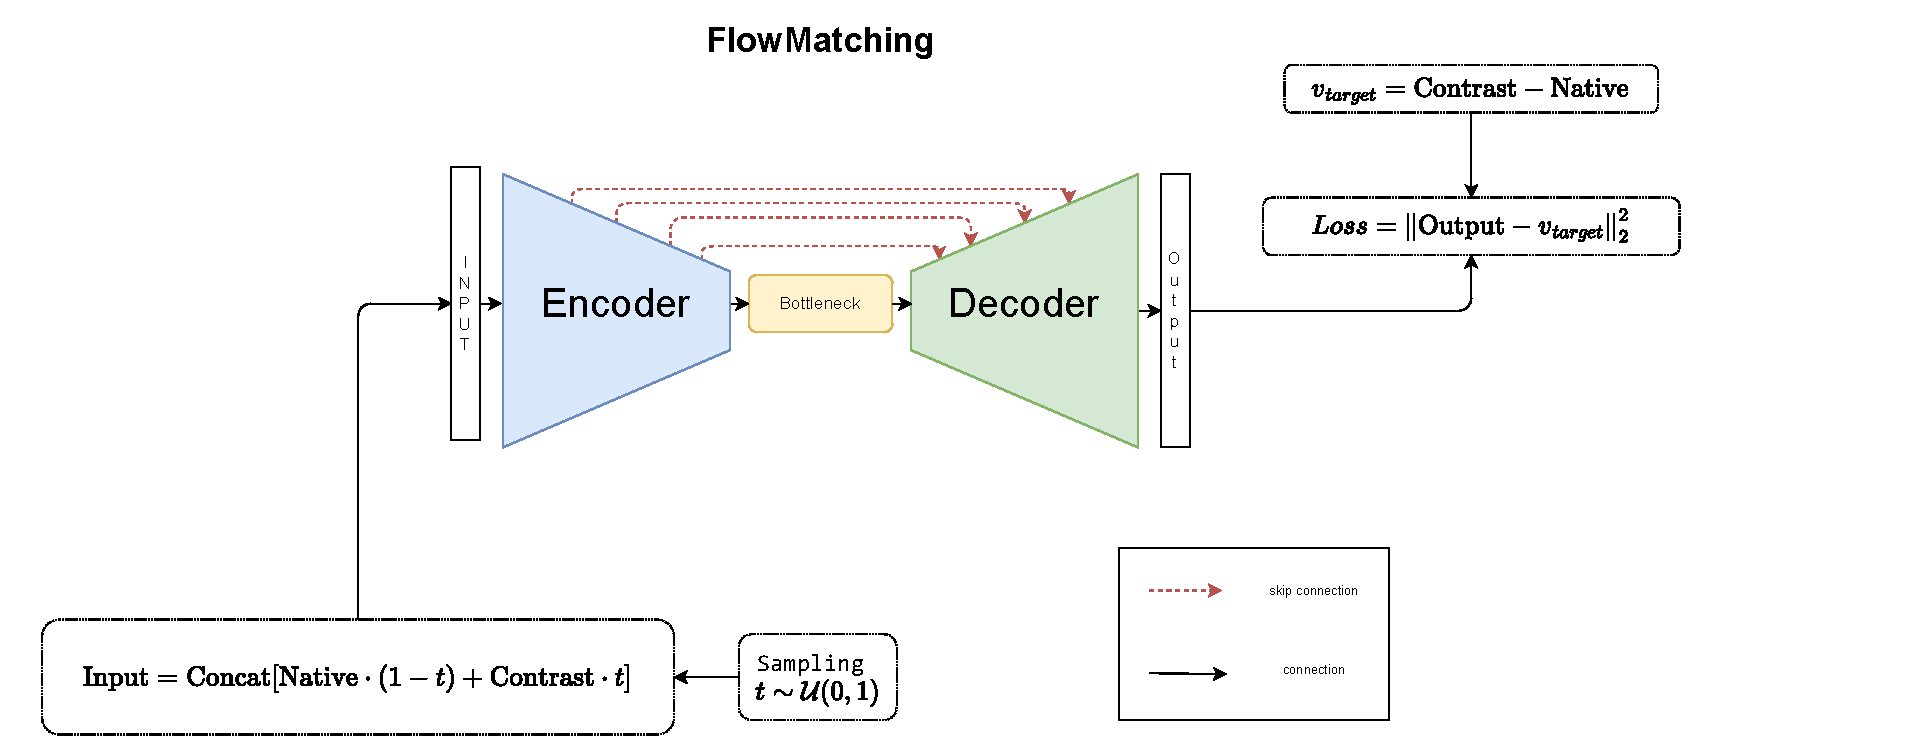
\includegraphics[width=\linewidth]{images/flow.pdf}
\end{frame}
% ------------------------------------------------------------------------

% ------------------------------------------------------------------------
\begin{frame}{TimeResNet}
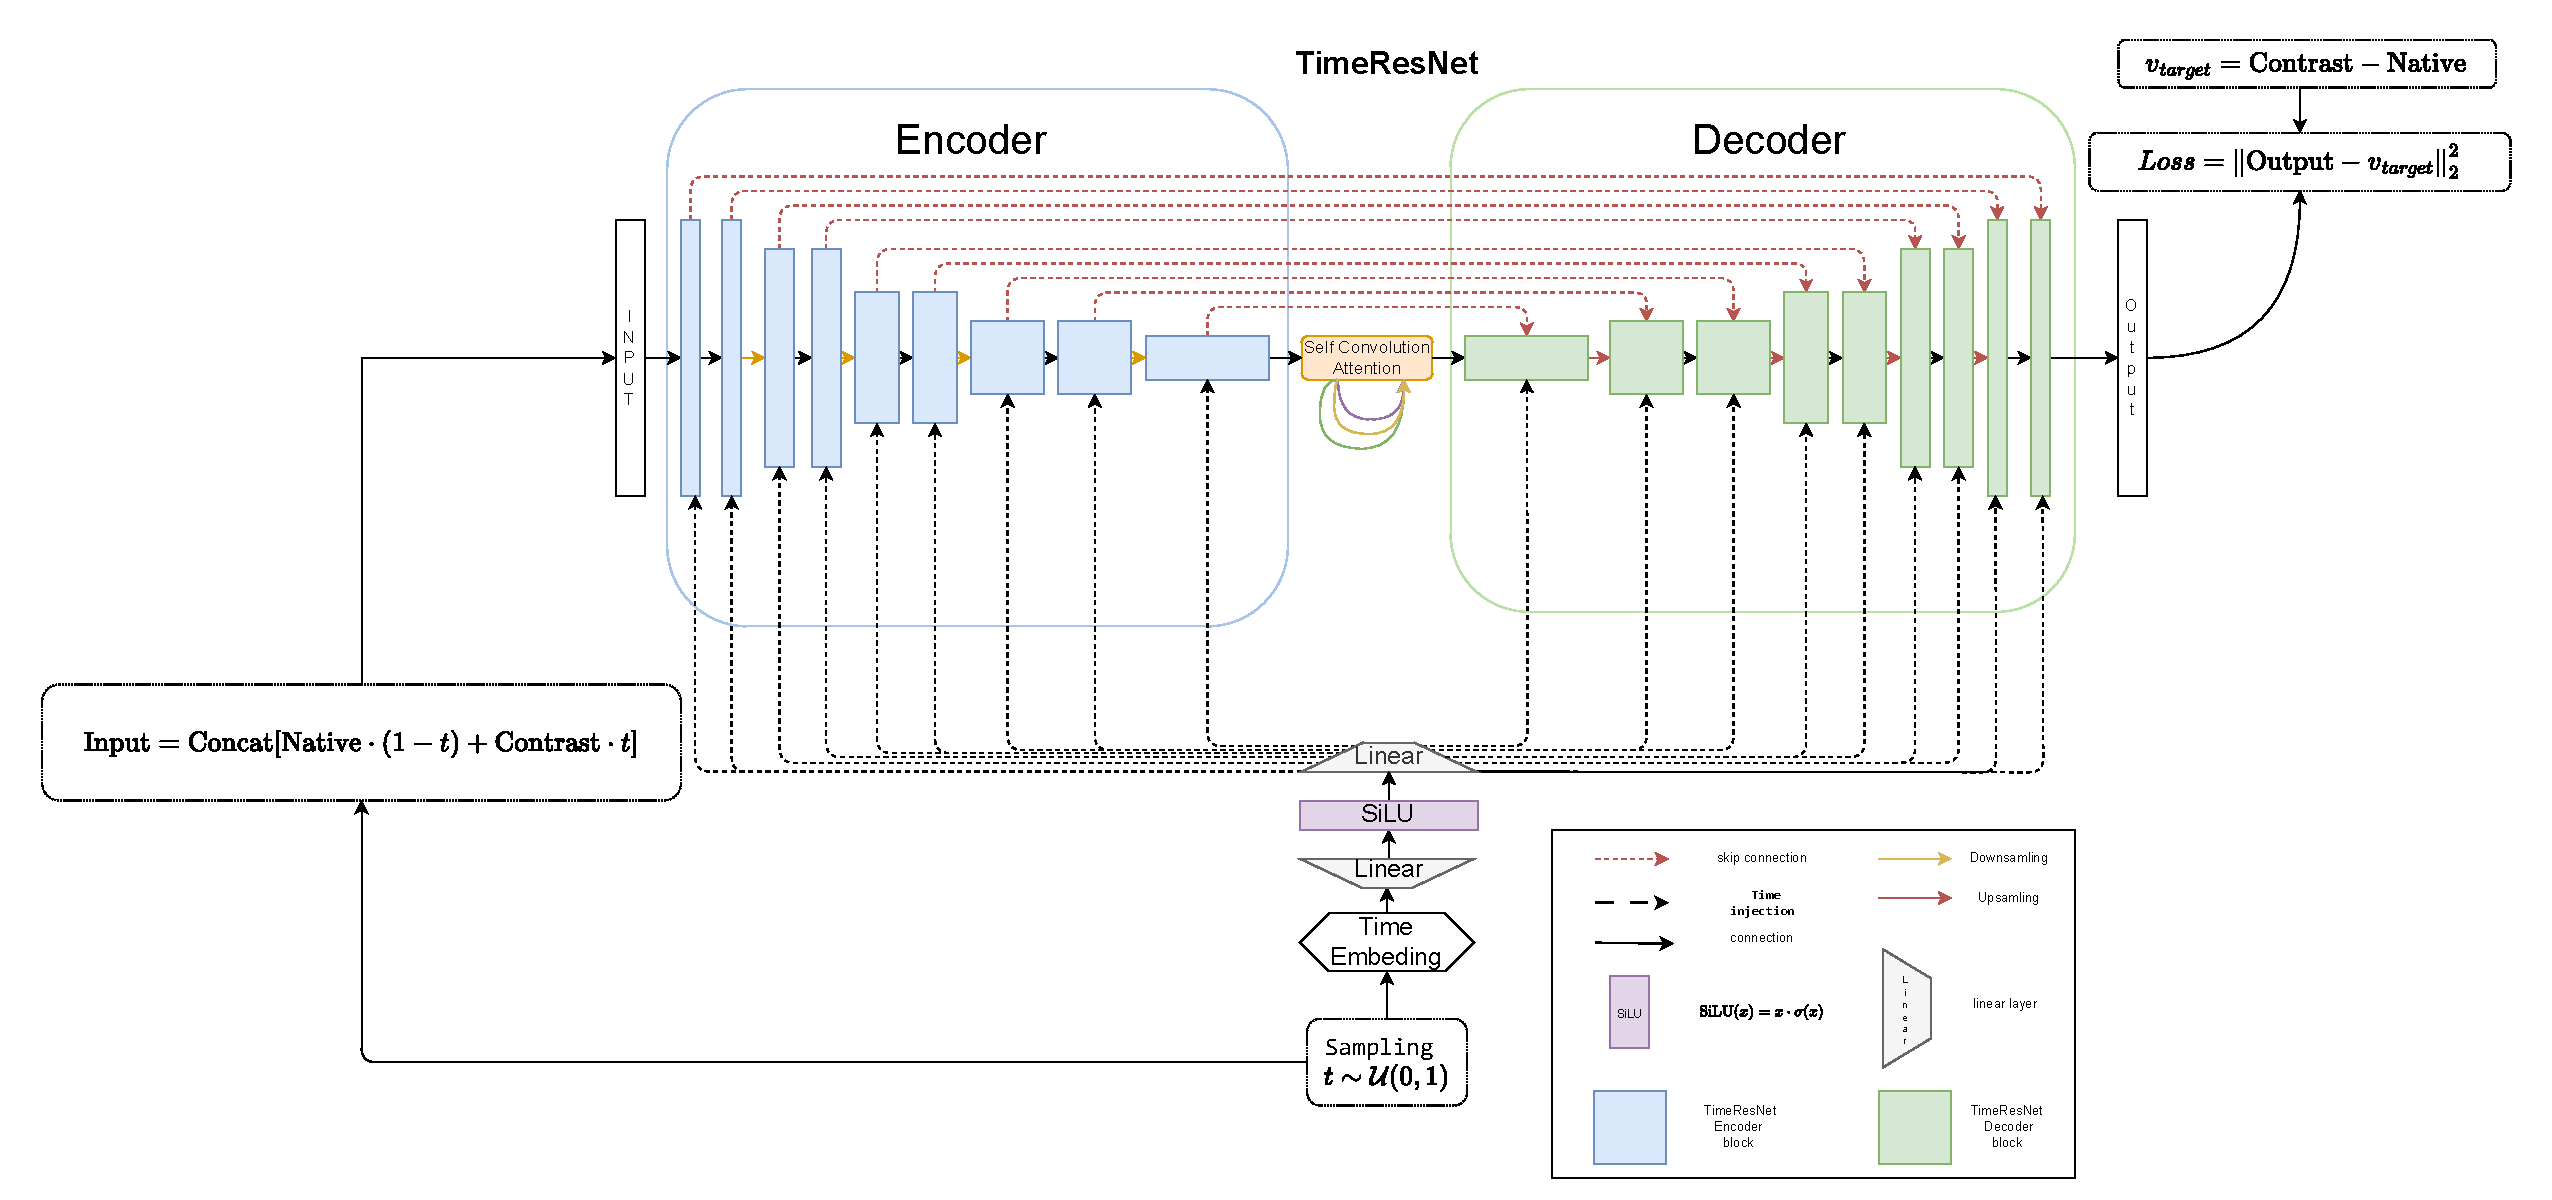
\includegraphics[width=\linewidth]{images/timeresnet.pdf}
\end{frame}
% ------------------------------------------------------------------------

% ------------------------------------------------------------------------
\begin{frame}{TimeResNetBlock}
\centering
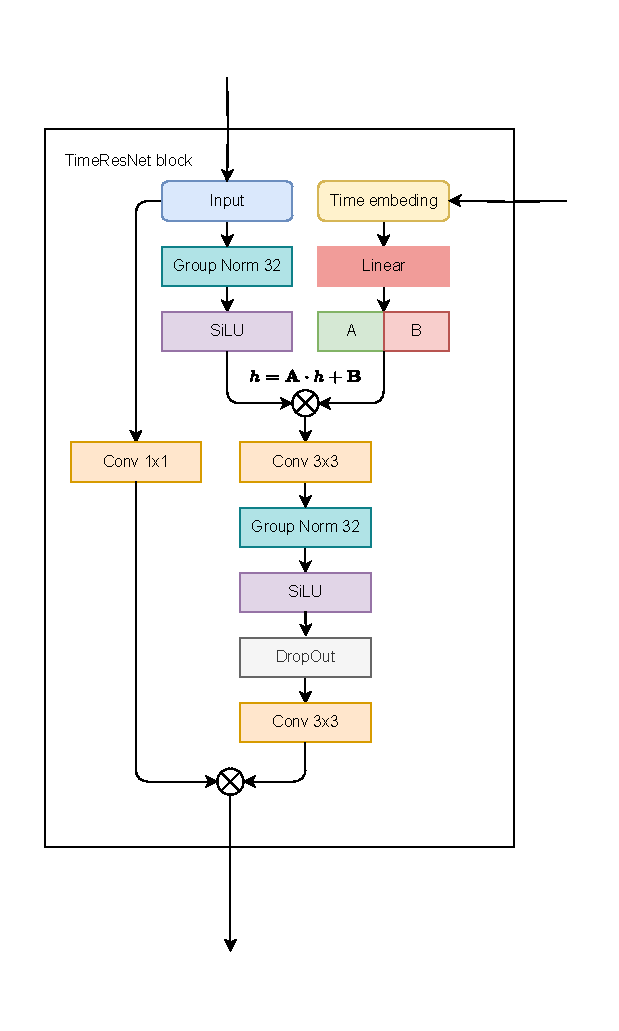
\includegraphics[scale=0.5]{images/Embeding.pdf}
\end{frame}
% ------------------------------------------------------------------------


% ------------------------------------------------------------------------
\begin{frame}{Постановка экперимента}
\begin{itemize}
\item \textbf{Задача:} аппроксимация векторного поля.
\item \textbf{Выборка:} 120 исследований (52561 2д изображений), 80 (34992) - обучение, 20 (8197) - тест, 20 (9372) - отложенная. 
\item \textbf{Архитектуры:} TimeResNet, DiffusionNet, SwinUNETR, SegResNet.
\item \textbf{Постановка эксперимента:}
\begin{enumerate}
    \item Регистрируем изображения с контрастом на изображения без контраста.
    \item Локализуем область исследования с помощью сегментации тела.
    \item Обрезаем картинку по (-1000, 1000) HU, переводим в (-1, 1).
    \item Сравниваем метрики и визуальные результаты с диффузией и регрессией.
\end{enumerate}
\end{itemize}
\end{frame}
% ------------------------------------------------------------------------

% ------------------------------------------------------------------------
\begin{frame}{Численные результаты}
\begin{table}[h!]
\centering
\renewcommand{\arraystretch}{1.15}
\begin{tabular}{lccccc}
\toprule
\textbf{Model} & MAE$\downarrow$ & SSIM$\uparrow$ & PSNR$\uparrow$ & Time, s$\downarrow$ & Params, M$\downarrow$ \\
\midrule
TimeResNet \textbf{(ours)} & \textbf{5.436} & \textbf{0.996} & \underline{39.776} & 0.209 & 124.7 \\
SwinUNETR         & 6.229 & \underline{0.992} & 38.933 & \underline{0.087} & \underline{120.1} \\
SegResNet         & \underline{6.146} & 0.983 & \textbf{40.108} & \textbf{0.056} & 214.1 \\
DiffusionNet         & 18.203 & 0.934 & 30.051 & 44.200 & \textbf{108.4} \\
\bottomrule
\end{tabular}
\label{tab:holdout_all}
\caption{Сравнение метрик моделей на hold-out выборке. TimeResNet и SwinUNETR обучены на задаче Flow Matching, SegResNet обучен на задачу регрессии, DiffusionNet обучен на задачу диффузии.}
\end{table}
\end{frame}
% ------------------------------------------------------------------------

% ------------------------------------------------------------------------
\begin{frame}{Выбор солвера}
    \begin{table}[h!]
\centering
\label{tab:solver_hold}
\renewcommand{\arraystretch}{1.15}
\begin{tabular}{lccccc}
\toprule
\textbf{Solver (steps)} & MAE$\downarrow$ & SSIM$\uparrow$ & PSNR$\uparrow$ & Time, s$\downarrow$ & Complexity \\
\midrule
Euler (1)      & 6.362 & 0.991 & 38.182 & \textbf{0.105} & 1 \\
Euler (2)      & 5.525 & 0.995 & 39.017 & \underline{0.210} & 2 \\
Euler (3)      & \underline{5.472} & 0.995 & 38.994 & 0.313 & 3 \\
Euler (5)      & 5.526 & 0.995 & 38.951 & 0.521 & 5 \\
RK2 (1)        & \textbf{5.436} & \textbf{0.996} & \textbf{39.776} & 0.209 & 2 \\
RK3 (1)        & 5.553 & 0.995 & 39.122 & 0.313 & 3 \\
RK4 (1)        & 5.716 & 0.995 & \underline{39.257} & 0.419 & 4 \\
Mid Point (1)  & 5.611 & 0.995 & 39.047 & \underline{0.210} & 2 \\
Mid Point (3)  & 5.759 & 0.995 & 38.923 & 0.628 & 6 \\
\bottomrule
\end{tabular}
\caption{Сравнение ODE-солверов для  TimeResNe на задаче (Contrast $\to$ Native) на \emph{hold-out}-выборке.}
\end{table}
% ------------------------------------------------------------------------

\end{frame}

% ------------------------------------------------------------------------
\begin{frame}{Визуальные результаты}
\centering
\includegraphics[scale=0.21]{images/small_example.png}
\end{frame}
% ------------------------------------------------------------------------

% ------------------------------------------------------------------------
\begin{frame}{Выносится на защиту}
\begin{itemize}
  \item Придуманы и имплементированы TimeResNet и TimeResNet block.
  \item Проведены значимые эксперименты, которые показывают что TimeResNet даёт преимущество по сравнению с нейронными сетями из фреймворка MONAI.
  \item Получена скорость генерации $\mathbf{400\times}$ быстрее диффузионных моделей, качество значительно превышает регрессию.
  \item На задаче сегментации, nnUNetV2 (фреймворк automl) на синтетических данных показывает Dice score $=0.926$ против $= 0.966$ на реальных данных.
  \item \textbf{Перспективы}: условная генерация образований в органах.
\end{itemize}
\end{frame}
% ------------------------------------------------------------------------

\end{document}
